% This is samplepaper.tex, a sample chapter demonstrating the
% LLNCS macro package for Springer Computer Science proceedings;
% Version 2.20 of 2017/10/04
%
\documentclass[runningheads]{llncs}
%
\usepackage{graphicx}
\usepackage{hyperref}
\usepackage{float}

\begin{document}
%
\title{Smart lecture rooms at universities}

\author{Group ID 07: Yunxuan Li \and
Zhixian Li \and
Jingxi Zhang}

\institute{Service Computing Department, IAAS, University of Stuttgart
\email{st119871,st146584,st141130@stud.uni-stuttgart.de}}
%
\maketitle              % typeset the header of the contribution
%
\begin{abstract}
This project is part of the lecture smart cities and internet of things \cite{ref_url1}. A lecture room is the most often and common place that student will go in an university. However, it is not easy to keep everyone in a lecture room comfortable, health and productive while have the lecture room itself secure and energy efficient. To achieve this goal, we plan to develop a smart lecture room system that uses different sensors to monitor the current state of a lecture room and automatically make decisions based on the information it has gathered.

\keywords{Lecture room  \and Smart building \and Comfortable \and Energy efficiency.}
\end{abstract}
%
%
%
\section{System Introduction}
For students, a lecture room might be the most often place we stay in an university. However, it’s hard to have everyone comfortable in a lecture room, for example, someone might want to have fresh air, but it could be too cold for others. In addition, it would be hard to keep everyone productive, for example, there might be a reflection on black board, but the professor did not notice. Furthermore, it could also be hard to keep the security and energy efficiency of a lecture room, for example, the door of a lecture could be left open and the light of a lecture room could be left on after a lecture is done. Besides, it is not necessary to run the HVAC devices at full capacity if the room is not occupied. Therefore, we want to develop a smart lecture room system that not only tries to make everyone in the room comfortable and productive but also keeps the lecture room secure and energy efficient. \\
To accomplish this goal, we decided to use different sensors in a lecture room that monitor the temperature, the weather, the air quality and so on. Based on these sensors, we will develop an automate system that decides when to make actions such like open the window or close the light. Also, with the use of calendar data the system is able to plan ahead to schedule the heating device or open the doors. Unfortunately, the system cannot carry out all these actions automatically due to limited hardware support. Thus, the decision will be sent to the professor or the room management so that they can do the corresponding actions.


\section{System Analysis}
We will describe the system functionality using user stories in the following, where these user stories will be the main focus of our project.
\begin{itemize}
\item As a lecturer I want the room to automatically adjust light and curtains, so that my powerpoint is clearly visible.
\item As a student or a lecturer I want the room temperature and humidity to be as ideal as possible for a lecture.
\item As a manager of the cost of the buildings I want the system to idealize the energy so that the cost is minimized.
\end{itemize}
 
These two user stories involve a door lock. As a physical door lock with electric mechanism is expensive we will stick to a simplification like sending an email or using a light to indicate the state of the door.
\begin{itemize}
\item As a caretaker of the building I want the doors to be locked after lecture hours so that the security of the building is able to be guaranteed. 
\item As a student I want the doors to be open before lecture to be able to prepare my utils for the lecture.\\
\end{itemize}

\section{System Architecture Design}
This section describes our system architecture. An overview of the architecture is shown in Figure \ref{fig:SystemArchitecture}.

\begin{figure}[H]
\centering
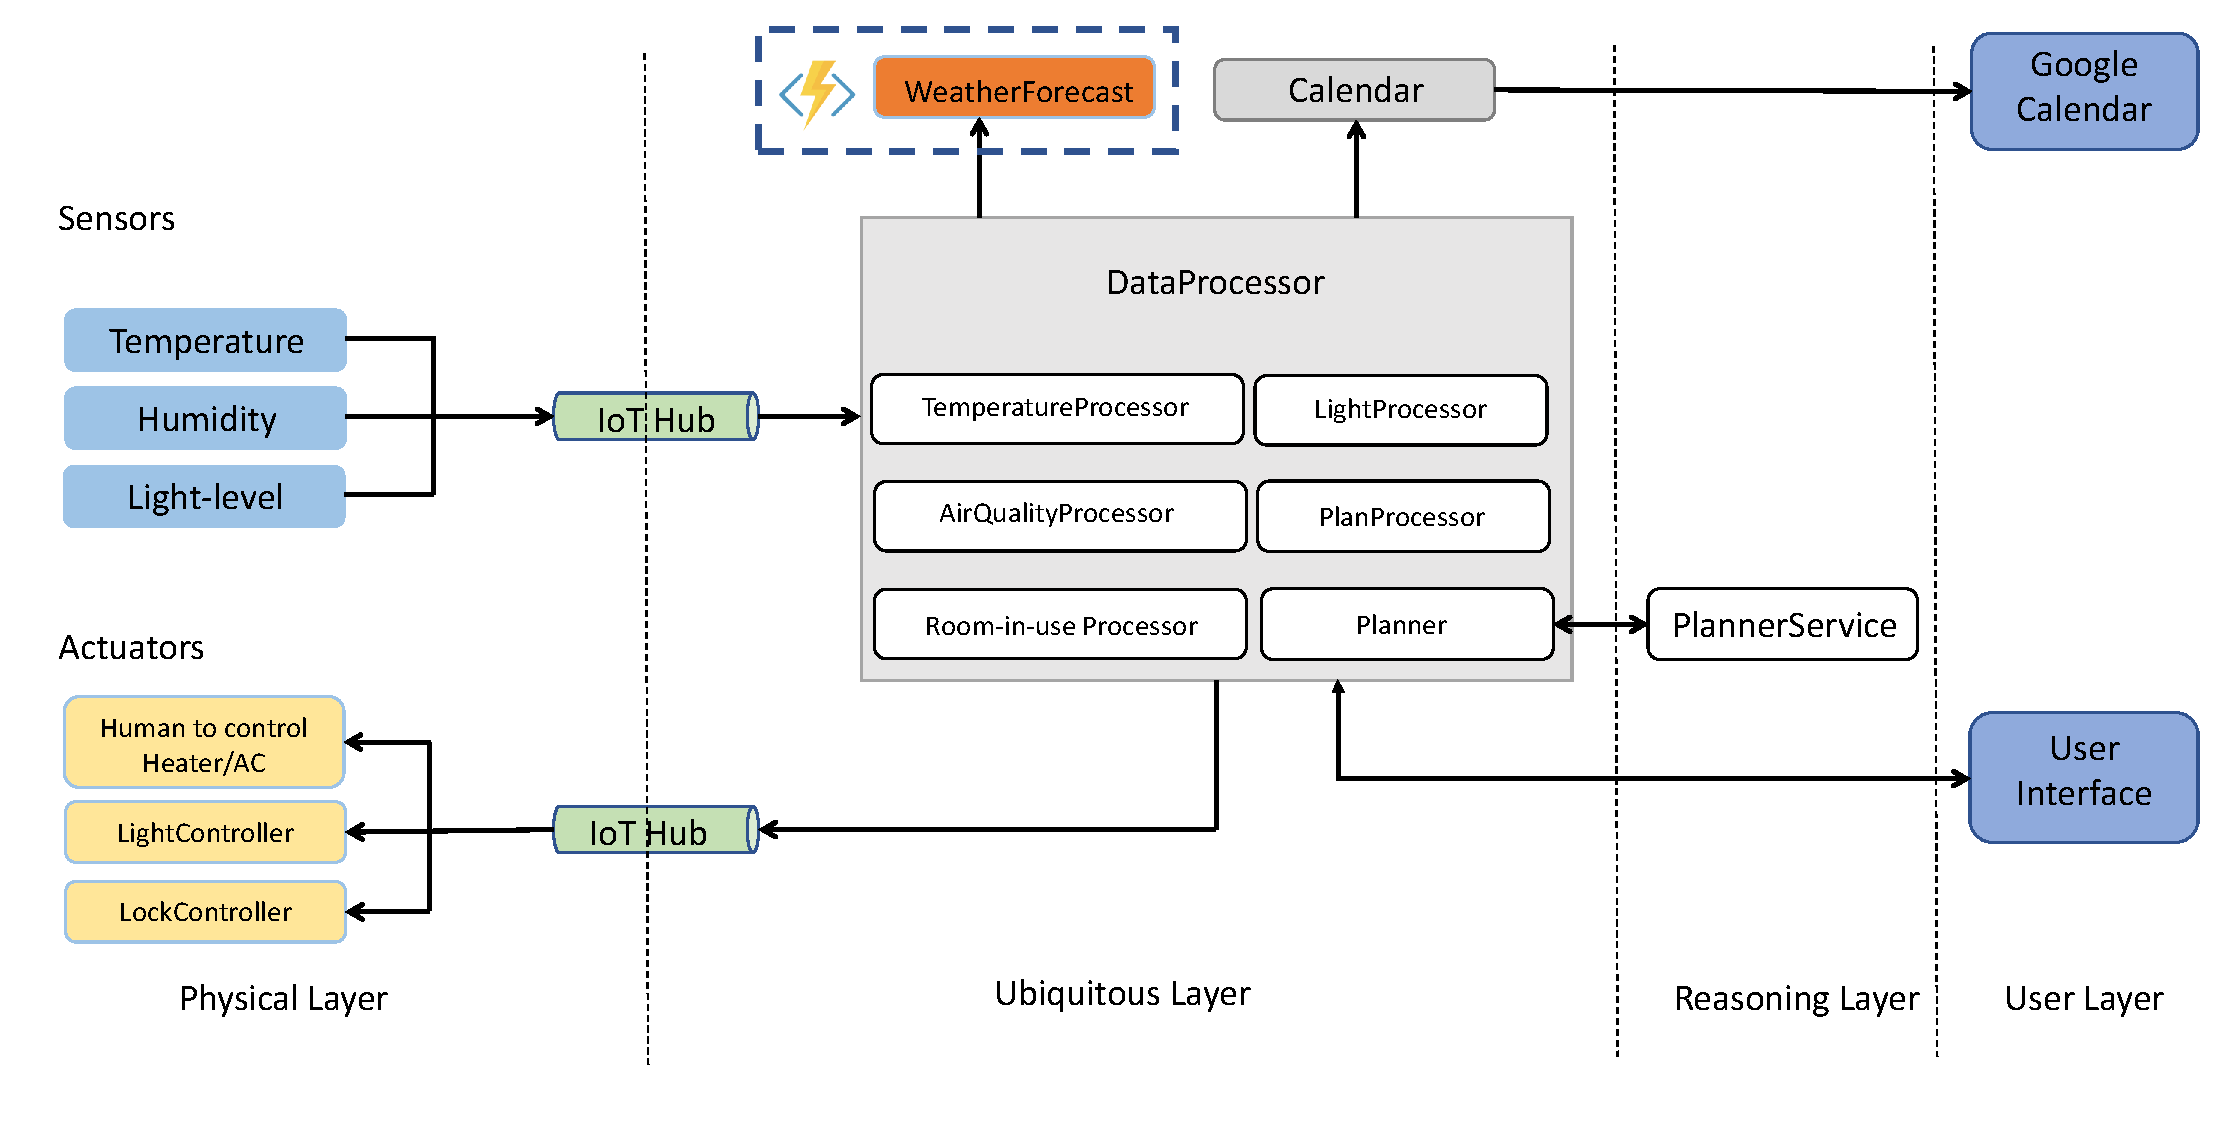
\includegraphics[width=1.0\textwidth]{../img/SystemArchitecture.pdf}
\caption{SystemArchitecture}
\label{fig:SystemArchitecture}
\end{figure}

The sensors at the physical layer are used to collect data like temperature and humidity of the lecture room and send them to the Data Processor through IoT Hub. Our Ubiquitous Layer will process the data received from the sensors and combine it with the weather forecast and calendar data. We have realized the weather forecast as an Azure function so that it can  directly be called when necessary. The Calendar component reads the Google Calendar and publishes the events to our Data Processor.\\
Our Planner service at the reasoning layer is the part where our AI planning comes into play. It makes a decision based on the data given. We use a PDDL Solver in the cloud \cite{solverpl71:online} as our planner, which is called via an HTTP request. The decision is forwarded to the actuators at the physical layer to carry out an action.\\
The actuators consists of controllers which adjust the light or lock automatically and humans who can execute actions upon request.\\
The user interface is realized on a laptop which communicates with a raspberry Pi where our system runs. In the user face light and air condition can also be manually adjusted.








%Components:


%Presentation layer\\
%Application logic layer\\
%Data layer \\

%
% ---- Bibliography ----
%
\bibliographystyle{splncs04}
\bibliography{mybib}

All links were last followed on \today

\end{document}
